\chapter{Introduction}
Speech recognition systems
started several decades ago.
They began with simple decoding capabilities through keyword
spotting and progressed to the modern Automatic Speech Recognition (ASR) systems
that are common nowadays\cite{asrBriefHistory}.

Recent advances in the field of speech recognition 
and acoustic modeling are
due to the introduction of 
Deep Neural Networks (DNN) 
based alternatives vice the traditional
Hidden-Markov Models---Gaussian Mixtures Models (HMM-GMM) 
approaches\cite{7472778, 6296526}.
With the introduction of DNN algorithms,
ASR systems performance significantly improved
compared to the conventional HMM-GMM 
based speech recognition approach\cite{7472778, 6296526}.
In addition, integration with deep beamformers,
which are also DNN-based, improves
the front-end (FE) performance in a way that is
eventually projected to lower error rates in results.
Different neural network (NN) 
architectures can be used to
implement ASR engine building blocks.
Usually, the NN used to train the ASR engine 
is the same NN used
in the implementation of the
front-end components, microphones, channel management,
and beamformers.

In recent years, the latest research 
interest has been in 
End-to-End (E2E) ASR systems\cite{boeddeker2018exploring}.
The E2E approach consists of the ``complete'' pipeline process, starting with
the audio domain physical signal reception up to the recognition engine.

\begin{figure}[H]
	\centering
	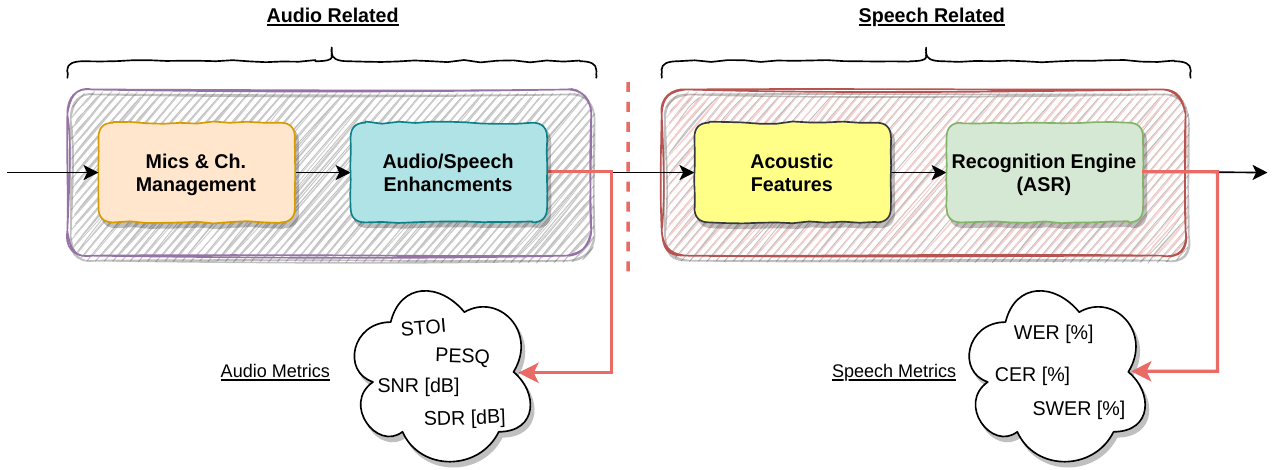
\includegraphics[width=\linewidth]{Introduction/images/asr_blocks}
	\caption{General E2E ASR System Blocks Diagram}\label{fig:asr_blocks_diagram}
\end{figure}
% \begin{figure}[H]
% 	\centering
% 	\includegraphics[width=0.99\textwidth]
% 	{./images/asr_blocks}
% 	\caption{General E2E ASR System Blocks Diagram}\label{fig:asr_blocks_diagram}
% \end{figure}
\vspace{-0.5cm}

Figure~\ref{fig:asr_blocks_diagram} shows 
a general skeleton of
an E2E ASR system. This general form describes the
internal partitioning and the pipeline process.
However, most importantly, it emphasizes
the distinction between the two domains of interest,
``Audio-related'' and ``Speech-related''.
These two domains are sometimes referenced
as ``Audio-Enhancement'' and ``Speech-Enhancement'', respectively.
Because there can be an overlap between
the two regions, ``Audio-related'' 
and ``Speech-related'' are probably the more precise terms.

% Notwithstanding the acknowledgment that 
% the name references describe each domain's 
% primary intention, they actually overlap.
% Therefore, ``Audio-related'' and ``Speech-related'' are more precise.
% Figure~\ref{fig:asr_blocks_diagram} shows what an End-to-End ASR system is
% generally constructed of. In addition, there is a non-strict distinction between
% two extensive areas in themselves. 


% Although overlap exists between the two domains,
The distinction between the two can be characterized
by different metrics.
Typically, speech-recognition performance is evaluated
using the Word Error Rate (WER) and
Character Error Rate (CER) metrics.
On the other hand, audio-related performance,
measured on the enhanced version of the input signal,
whether it be speech separated or noise suppressed,
is evaluated using different metrics.
If such audio enhancement processing is applied,
metrics like Clarity, Definition,
Reverberation-Time, and other standard signal processing metrics
such as Signal to Noise Ratio (SNR) 
and Signal to Distortion Ratio (SDR) are used.

% Although there is a kind of distinction between these two domains of interest, sometimes the
% distinction line is not strongly put between the ``speech enhancements'' to the ``acoustic features''
% building blocks, nor the requirement to have all these components in an E2E ASR system.

% \bigskip

% With that said, it is still very important
% to distinguish between the different metrics
% that are used to evaluate the performance of such systems. Where speech-recognition related 
% performance is mostly evaluated using the Word Error Rate (WER) and Phone Error Rate (PER) metrics.

% \bigskip

% On the other hand, audio related performance,
% which is measured on the ``enhanced'' version
% of the input signal (if such processing is applied),
% is evaluated using different metrics like 
% Clarity (C50), Definition (D50), Reverberation-Time (T50) 
% and other common signal processing metrics
% as Signal to Noise Ratio (SNR) and Signal to Distortion Ratio (SDR).

\bigskip

In turn, the first building block of the 
``Audio-related'' part that is called 
"Microphones \& Channels Management" as shown 
in Figure~\ref{fig:asr_blocks_diagram},
can be evaluated with 
different sets of performance metrics 
such as Directivity Factor (DF),
Noise Gain (NG) and more.

Compared to a reference and a specific performance metric, 
a change in any of the building blocks 
shown in Figure~\ref{fig:asr_blocks_diagram} may 
improve or degrade performance. 
On the other hand,
performance increase in one metric can cause 
a degradation in other metrics.
Hence, some cross-correlation and trade-off estimations
over the given metric constrains should be performed
before and during the design stage of an E2E ASR system. 
The outcomes may pour light on what would be a better
and sufficient solution for a given usecase. 
Furthermore, other performance metrics can be examined.
For example, metrics like computation time and resources utilization
can assist in having a more comprehensive overview of how the system operates given a
static pipeline with different algorithms.
Thus, application
developers can benefit from such metrics estimations,
especially when dealing with strict 
application requirements or resource-limited platforms.
% \bigskip

% With the introduction of DNN algorithms,
% E2E ASR systems performance significantly improved
% compared to the conventional HMM-GMM 
% based speech recognition approach\cite{7472778, 6296526}.
% In addition, integration with deep beamformers,
% which are also DNN-based, improves
% the front-end performance in a way that is
% eventually projected to lower WER results.

% \bigskip

% Different neural network (NN) 
% architectures can be used to
% implement of ASR engine building blocks.
% Usually, the NN used to train the ASR engine 
% is the same NN used
% in the implementation of the
% front-end components, microphones, channel management,
% and beamformers.

% in the implementation of the front-end components 
% the same NN is used in the front-end components, Microphones, channel management, and beamformers.

% Different neural network architectures can be applied for
% both the recognition engine, i.e. ASR building block,
% and the front-end components, i.e. Microphones, channel management, and beamformers.

\bigskip

% Compared to a reference and a specific performance metric, 
% each change might improve performance. 
% On the other hand,
% performance in one metric can cause degradation in other metrics.
% Hence, some cross-correlation and trade-off estimations
% should be performed before an E2E ASR system design stage.
% Furthermore, other performance metrics can be embraced.
% For example, metrics like computation time and resources utilization
% can assist in having a more comprehensive overview of how the system operates given a
% static pipeline with different algorithms.
% Thus, application
% developers can benefit from such metrics estimations,
% especially when dealing with strict 
% application requirements or resource-limited platforms.

% when their platforms have limited resources, or when 
% their application requirement are strict.
% for such metrics can be useful for application
% developers, who target for resource limited platforms 
% or are constrained to specific application requirements. 

\section{Literature Review}
References~\cite{7472778, 7952160} are 
two pioneering research papers focusing on 
studying neural networks usages
for beamforming in the front-end, right
before the acoustic features extraction and
recognition engine stages in E2E ASR systems.
In both papers, the researchers built their architecture
upon the principles of an E2E ASR pipeline.
Those architectures share a similar baseline but have different
DNN-type beamformers, filters, and ASR engines.
Experiments in ~\cite{7472778, 7952160}
focus on WER performance evaluations to express
the system's capabilities under 
different test-cases and inputs.
Few of the test-cases, for example, are a single microphone 
with single channel input,
a single microphone with multi-channel inputs,
and a microphones array.
% \begin{figure}[H]
% 	\centering
% 	\begin{subfigure}[b]{0.41\textwidth}
% 		\includegraphics[width=\textwidth, keepaspectratio=true]
% 		{./images/gcc_dnn_BF_blocks}
% 		\caption{System Architecture Used In~\cite{7472778}}\label{fig:gcc_dnn_BF_blocks}
% 	\end{subfigure}
% 	\begin{subfigure}[b]{0.55\textwidth}
% 		\includegraphics[width=\textwidth, keepaspectratio=true]
% 		{./images/lstm_BF_blocks}
% 		\caption{System Architecture Used In~\cite{7952160}}\label{fig:lstm_BF_blocks}
% 	\end{subfigure}
% \end{figure}

% \bigskip

% Experiments in ~\cite{7472778, 7952160}
% focus on WER performance evaluations to express
% the system's capabilities under 
% different test-cases and inputs.
% Naming few, a single microphone 
% with single channel input,
% a single microphone with multi-channel inputs,
% and a microphones array.

% \bigskip

\subsection{Recent Work}
Recently, new techniques have been introduced~\cite{900384911,20202222222,9003849,7471664,8466865},
such as
different NN architectures that serve as the basis for
the ASR engines.  
% \begin{itemize}[noitemsep]
% 	\item ASR Engine alternatives
% 	\item biasing
% 	\item Low Latency Beamformers
% 	\item Masking operations
% \end{itemize}

\subsubsection{ASR Engine Alternatives}
Performance comparisons between different recognition
engines are described in~\cite{900384911}. 
The different ASR engines include 
Recurrent neural network-transducer (RNN-T), 
Recurrent neural network-attention encoder decoder (RNN-AED),
and Transformer-AED.
These architectures belong to the right side
of the extended E2E ASR structure shown in 
Figure~\ref{fig:asr_blocks_diagram}, 
also referred to as the
Back-end (BE).
BE engines are complex systems by themselves
and thus can be split into multiple smaller
blocks to ease integration.
Despite being very comprehensive, reference~\cite{900384911} 
concentrates on
the ``Speech related'' domain,
such that the primary metric used for evaluation is WER,
without considering the front-end
effect and its correlation to performance.
In addition, the recognition engines in this paper
do not make use of the 
Listen, Attend, and Spell (LAS)~\cite{7472621}
nor the Connectionist Temporal 
Classification (CTC)~\cite{hannun2017sequence},
which are now considered as integral components in modern 
ASR engines after proving to enhance recognition rates drastically. 
% \bigskip

% In~\cite{900384911}, the primary metric used for evaluation is WER.
% The different ASR engines include 
% Recurrent neural network-transducer (RNN-T), 
% Recurrent neural network-attention encoder decoder (RNN-AED),
% and Transformer-AED.
% These architectures belong to the right side
% of the extended E2E ASR structure shown in 
% Figure~\ref{fig:asr_blocks_diagram}, 
% also referred to as the
% Back-end (BE).
% BE engines are complex systems by themselves
% and thus can be split into multiple smaller
% blocks to ease integration.
% Despite being very comprehensive, this research paper 
% concentrates on
% the ``Speech related'' domain
% without considering the front-end
% effect and its correlation to performance.

\subsubsection{Biasing}
Reference~\cite{20202222222} explores the effect of biasing
on a complete E2E ASR system pipeline. 
First, masking operations were
applied in the frequency domain.
Then, biasing information was fed
into the system in combination with the 
masked frequency output. 
The added biasing information
together with the T-F masking and the beamformer
in the front-end showed a substantial reduction
in error rate detections.

% \begin{figure}[H]
% 	\centering
% 	\includegraphics[width=0.99\textwidth]
% 	{./images/e2e_bias_blocks}
% 	\caption{System Architecture Used In~\cite{20202222222}}\label{fig:e2e_bias_blocks}
% \end{figure}


\subsubsection{Low Latency Beamformers}
Low latency beamformers were studied in~\cite{9003849}.
The research results show 
"audio-related" performance comparisons
as a function of the beamformer type and the number
of microphones in the array.
Moreover, each setup's latency was measured to determine 
its time to process. 
The authors of this paper used
two different datasets for their experiments.
The TIMIT dataset~\cite{timitDS} for the generations of noisy reverberant
inputs to the microphone array and the CHiME 3~\cite{chime3DS} dataset
for ASR evaluations.


\subsubsection{Masking Operations}
Reference paper~\cite{7471664} demonstrates experiments on estimations of spectral masks effects
with neural networks based beamformers.
Two different beamformers,  Generalized Eigenvector (GEV)
and Minimum Variance Distortionless Response (MVDR) were tested with and without Bi-directional Long Short-Term Memory (BLSTM)
spectral masks concerning the Power Spectral Distribution (PSD)
and SNR.
However, this paper does not include an E2E pipeline nor the recognition engine.
In other words, this research focuses on the ``Audio-related'' domain.
Indeed, SNR belongs to the
``Audio-related' metric set rather than the
``Seech-related'' metric set,
as shown in Figure~\ref{fig:asr_blocks_diagram}.
\bigskip

Another comprehensive research 
that studies masking operations
is described in~\cite{8466865}.
In this paper, the architecture does not include
the ASR engine. 
Instead, it mainly deals with the enhanced output signal,
signifying that it is also in the ``Audio-related'' domain.
However, this research is unique in that
it utilized both the WER and SDR metrics measurements
for different engines that were plugged in at the BE stage.

% \begin{figure}[H]
% 	\centering
% 	\includegraphics[width=0.75\textwidth]
% 	{./images/robust_mask_blocks}
% 	\caption{System Architecture Used In~\cite{8466865}}\label{fig:robust_mask_blocks}
% \end{figure}

% Here, the engine is not present in the architecture, but only the enhanced 
% output signal which is also in the ``Audio related'' domain.

\section{Project Outline}
Applications have requirements and limitations
that are dictated by their platform or available hardware.
A way to estimate Hardware (HW) requirements for speech
applications based on speech-related or audio-related metric sets
can be helpful to developers of such platforms.
Therefore, optimizations of a given E2E ASR architecture by careful
trade-off selections can lead to more robust and rapidly
developed applications or setups.
That is a significant advance towards fast setup constructions for different HW platforms.
As such, in this thesis, the effects of changing different
building blocks and applying various enhancement techniques
in a given E2E ASR system will be evaluated.
The effects of such replacements and
fine-tunes will be presented with respect to different
performance metrics. Based on the results, one will be able to deduce the trade-offs
that can be selected to optimize the implementation process for a specific
application, platform, requirement, feasibility, and other specifications.

\bigskip

Evaluated performance metrics
are shown in Figure~\ref{fig:metrics_cross_blocks}
% , where the goals of the research are
% to produce a cross-correlation between the different
% metric sets and trade-offs that can be used to select an optimal design.

\begin{figure}[H]
    \centering
    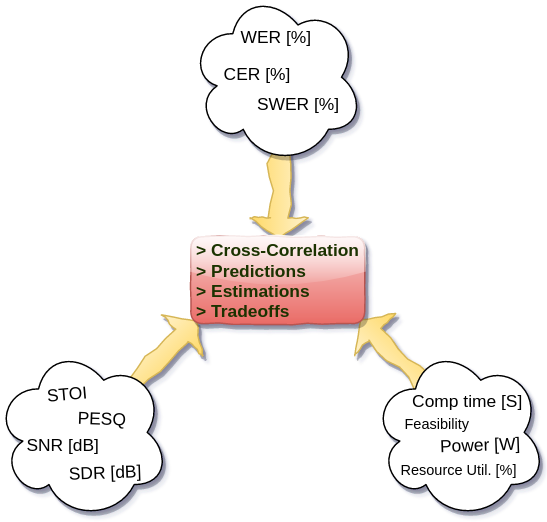
\includegraphics[width=0.75\linewidth]{Introduction/images/metrics_cross_blocks}
    \caption{Project Outline Summary Diagram}\label{fig:metrics_cross_blocks}
\end{figure}
% \begin{figure}[H]
% 	\centering
% 	\includegraphics[width=0.7\textwidth]
% 	{./images/metrics_cross_blocks}
% 	\caption{Project Outline Summary Diagram}\label{fig:metrics_cross_blocks}
% \end{figure}

A comprehensive performance metrics table that contains the Audio,
Speech, and HW characteristics
of an E2E ASR system, will be composed.
Such tables make it easier to detect cross-correlations between the metric sets.
In consequence, 
deduction of each metric's
projection on others can be estimated.

% Hardware metrics estimations based on the other metric sets
% can be useful for application developers. Usually applications have requirements 
% and limitations that are constrained to their platform or available hardware.
% Therefore, some trade-offs

% \bigskip


% that can be selected in order to optimize a given E2E ASR
% architecture can lead to more robust and rapidly developed applications or setups.
% That is a big advance towards fast setup constructions for different hardware platforms. 


% In this research project, I want to study the effects as described in the project outline section.
Our approach is to setup an architecture 
that follows the entire E2E ASR pipeline including
the beamforming FE as presented in
Figure~\ref{fig:proj_blocks}.
% but also includes 
% masking operations 
% Figure~\ref{fig:e2e_bias_blocks}, with some changes that will be described below. 
% The system should follow the baseline pipeline as shown in 
% Figure~\ref{fig:gcc_dnn_BF_blocks} and Figure~\ref{fig:lstm_BF_blocks}.
\begin{figure}[H]
	\vspace{-2.65cm}
	\centering
	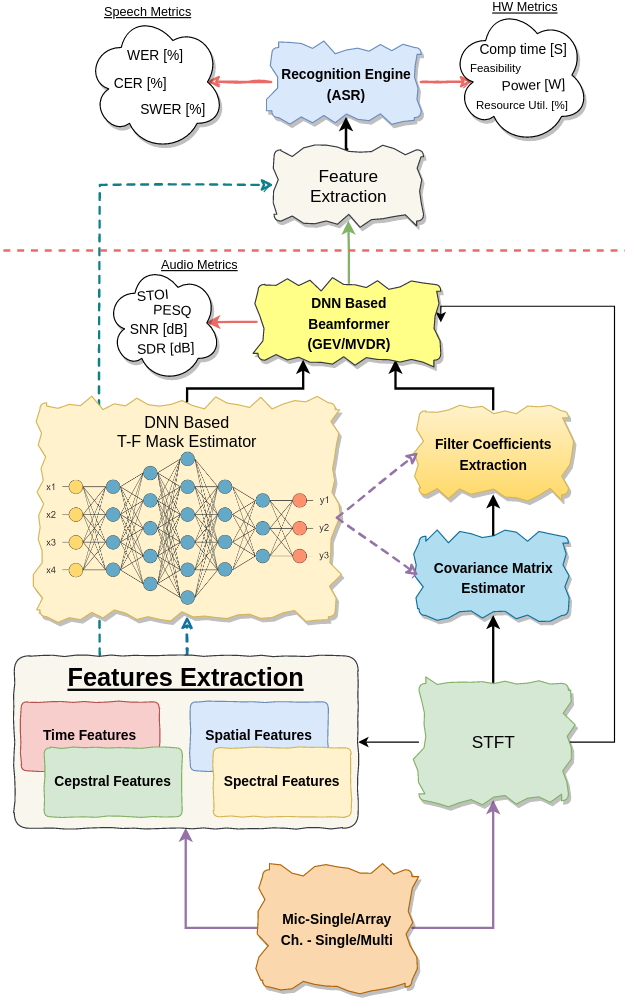
\includegraphics[width=\textwidth]
	{Introduction/images/proj_blocks2}
	\caption{Project's Architecture}\label{fig:proj_blocks}
\end{figure}



This paper's structure follows the architecture
presented in Figure~\ref{fig:proj_blocks}.
In Chapter~\ref{ch:metrics}, 
we introduce the selected performance evaluation metrics
of interest and how they relate to these domains. 
A detailed explanation of how each performance metric is
extracted and calculated is provided as well
for a better understanding of the motivation behind
these metrics selection.

Chapter~\ref{ch:scaling_methods} describes three different scaling methods
that are commonly used in audio processing and analysis.
We also present detailed performance comparisons in this chapter based on
the evaluation metrics that we described in Chapter~\ref{ch:metrics}.

The understanding of audio frequency scaling and 
the differences between scaling methods
are essential for Chapter~\ref{ch:features}. 
Key features analysis is given in this chapter along with
the considerations and the importance of every feature
for the sake of accurate speech classification and audio processing. 

Chapter~\ref{ch:tf_mask_ch} surrounds Time-Frequency (TF) 
masking techniques which is a preliminary process taken prior
to beamforming. 
In this chapter, we cover four
dominant masking technique, starting with background theory,
through implemntation to measured performance evalutaions.
The T-F masking outputs are dynamically estimated
by a DNN subsystem 
and serve as the input weights
to a beamformer that is connected next.

Beamforming concepts and 
common beamforming architectures for speech
are described in Chapter~\ref{ch:beamformers}.
This chapter follows the T-F masking chapter
since it actually work on the outputs that are produced
by the T-F masking DNN system.

General background about 
ASR systems is given in
Chapter~\ref{ch:asr_ch}.
After that we go thorugh history in the evolvment process
of ASR systems to what we know today as E2E ASR system.
We emphasize the benefits of using E2E solutions
and what other advancements were done in this field of research.
Then, we present our general approach of an ASR engine implementation,
followed by multiple variants of 
suggested ASR engines and their measurement evaluations.

Chapter~\ref{ch:datasets} describes the datasets that
we use for training and evaluations of our various
DNN systems. We make use of the multi-microphone CHiME datasets~\cite{chime3DS}
for the T-F masking and beamforming parts, 
and the CommonVoice V7 dataset~\cite{commonVoiceDS}
for the ASR engine module.

In Chapter~\ref{ch:concl_ch}, we provide conclusions to the study
and our plan for future work.